\documentclass[a4paper]{article}
\usepackage[14pt]{extsizes}
\usepackage[T2A]{fontenc}
\usepackage[utf8]{inputenc}
\usepackage[russian]{babel}
\usepackage{setspace,amsmath}
\usepackage{graphicx}
\usepackage{epigraph} 
\usepackage{csquotes} 
\usepackage[unicode, pdftex]{hyperref} 
\usepackage{amssymb} 
\usepackage{caption}
\usepackage{amsthm} 
\usepackage{wrapfig}
\usepackage[table,xcdraw]{xcolor}
\usepackage[left=15mm, top=10mm, right=10mm, bottom=15mm, nohead, footskip=10mm]{geometry} 
\RequirePackage{caption}
\DeclareCaptionLabelSeparator{d}{}
\captionsetup{justification=centering,labelsep=d}

\begin{document}
\title{\textbf{Лабораторная работа 1.3.3}

\

Измерение вязкости воздуха по течению в тонких трубках
\
}
\author{Д. Лежнев, И. Артемов}
\date{\today}
\maketitle
\noindent
\textbf{Цель работы:} экспериментально исследовать свойства течения газов по тонким трубкам при различных числах Рейнольдса; выявить область применимости закона Пуазейля и с его помощью определить коэффициент вязкости воздуха.

\noindent
\textbf{Оборудование:} система подачи воздуха (компрессор, подводящие трубки); газовый счетчик барабанного типа; спиртовой микроманометр с регулируемым наклоном; набор трубок различного диаметра с выходами для подсоединения микроманометра; секундомер.

\section*{1. Теоретическое введение.}
Работа посвящена изучению течения воздуха по прямой трубе круглого сечения. Движение жидкости или газа вызывается перепадом внешнего давления на концах $\Delta P$ трубы, чему в свою очередь препятствуют силы вязкого
(«внутреннего») трения, действующие между соседними слоями жидкости, а также со стороны стенок трубы.

\noindent
Характер течения в трубе может быть ламинарным либо турбулентным.
При ламинарном течении поле скоростей $\vec{u}(\vec{r})$ образует набор непрерывных
линий тока, а слои жидкости не перемешиваются между собой. Турбулентное течение характеризуется образованием вихрей и активным перемешиванием слоев, при этом даже в стационарном течении в каждой точке имеют место существенные флуктуации скорости течения и давления.

\noindent
Характер течения определяется числом Рейнольдса:
\[Re = \frac{\rho u a}{\eta} ,\]
где $\rho$ - плотность среды, $u$ - характерная скорость потока, $a$ - характерный размер системы, $\eta$ - вязкость среды. Число Рейнольдса показывает отношение кинетической энергии элемента объёма жидкости к потерям энергии на трение $K/A_{fr}$. При малых значениях Re в потоке доминируют вязкие силы трения, и движение ламинарно. При значениях Re, больших некоторого критического ($\sim 10^3$), характер течения меняется на турбулентный.

\noindent
В нашей модели также будет считаться, что газ \textit{несжимаем} ($\rho = const$), что допустимо, так как относительный перепад давления $\Delta P/P \ll 1$, а скорость течения газа много меньше  скорости звука в нём.

\subsection*{Течение Пуазейля.}
Рассмотрим движение жидкости при малых Re. Оно будет ламинарным, поэтому в любом сечении трубки давление одинаково, а скорость течения среды $\vec{\upsilon}$ всюду направлена вдоль оси трубы. 

\noindent
Из 2 закона Ньютона для цилиндра жидкости длиной $dx$ и радиусом $r$, имеющем координату $x$ (рис. 1):

\begin{figure}
\center{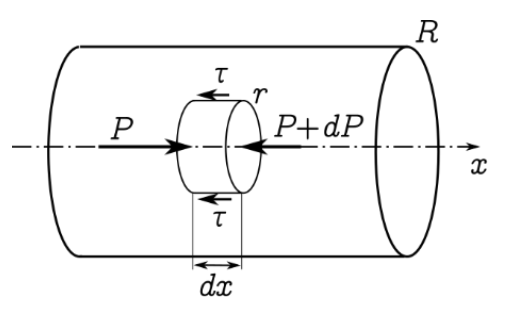
\includegraphics[scale=1]{рис 1.png}}
\caption{\textit{. К выводу формулы Пуазейля.}}
\end{figure}

\[\pi r^2 dP = -\eta \frac{d\upsilon}{dr} 2\pi r dx \Rightarrow \frac{dP}{dx} = -\frac{2\eta}{r} \frac{d\upsilon}{dr}\]
Левая часть выражения зависит только $x$, правая	 зависит только от  $r$, поэтому обе части выражения являются константами. Тогда:
\begin{equation}
P(x) = P_0 - \frac{\Delta P}{l}x,
 \end{equation} 
где $P_0 = P(0)$, $\Delta P$ - перепад давления на участке длиной $l$. 

\noindent
Для скорости имеем:
\[\upsilon(r) = \upsilon(0) - \frac{\Delta P}{4 \eta l}r^2  \]
Используя граничное условие $u(R) = 0$, получим:
\begin{equation}
\upsilon(r) = \frac{\Delta P}{4\eta l} (R^2 - r^2) 
\end{equation}
Тогда объёмный расход жидкости:
\begin{equation}
Q = \int\limits_{0}^{R} \upsilon(r) 2\pi r dr = \frac{\pi R^4 \Delta P}{8 \eta l}
\end{equation}
Средняя скорость потока:
\begin{equation}\label{eq4}
u \equiv \overline{\upsilon} = \frac{Q}{\pi R^2} = \frac{R^2 \Delta P}{8 \eta l}
\end{equation}

\subsection*{Длина установления.}
Пусть на вход трубы поступает течение, распределение которого не является пуазейлевским. Определим длину $l_{est}$, на которой установится пуазейлевское течение. 

\noindent
Кинетическая энергия цилиндра толщиной $dx$:
\[K \sim \frac{1}{2} \rho u^2  \pi R^2 dx \]
Работа сил трения на длине $l$:
\[A_{fr} \sim \eta \frac{u}{R} \cdot 2\pi r \cdot dx \cdot l\]
Если $l = l_{est}$, то $A_{fr} \sim K$, поэтому:
\[l_{est} \sim \frac{\rho u R^2}{\eta}  = R \cdot Re\]
Из опыта:
\begin{equation}\label{eq5}
l_{est} = 0.2 R \cdot Re 
\end{equation}
Экспериментально $l_est$ можно будет определить, измеряя распределение давления вдоль оси трубки $P(x)$. На неустановившемся участке будет наблюдаться отклонение от линейного закона и при том же расходе $Q$ градиент давления будет больше (ибо участки жидкости имеют ускорение).

\section*{2. Экспериментальная установка.}
\noindent
Схема экспериментальной установки изображена на рис. 2. Поток воздуха под давлением, немного превышающим атмосферное, поступает через газовый счётчик в тонкие металлические трубки. Воздух нагнетается компрессором, интенсивность его подачи регулируется краном К. Трубки снабжены
съёмными заглушками на концах и рядом миллиметровых отверстий, к которым можно подключать микроманометр. В рабочем состоянии открыта заглушка на одной (рабочей) трубке, микроманометр подключён к двум её выводам, а все остальные отверстия плотно закрыты пробками.

\

\noindent
Перед входом в газовый счётчик установлен водяной U-образный манометр. Он служит для измерения давления газа на входе, а также предохраняет
счётчик от выхода из строя. При превышении максимального избыточного
давления на входе счётчика ($\sim$ 30 см вод. ст.) вода выплёскивается из трубки
в защитный баллон Б, создавая шум и привлекая к себе внимание экспериментатора.

\begin{figure}
\center{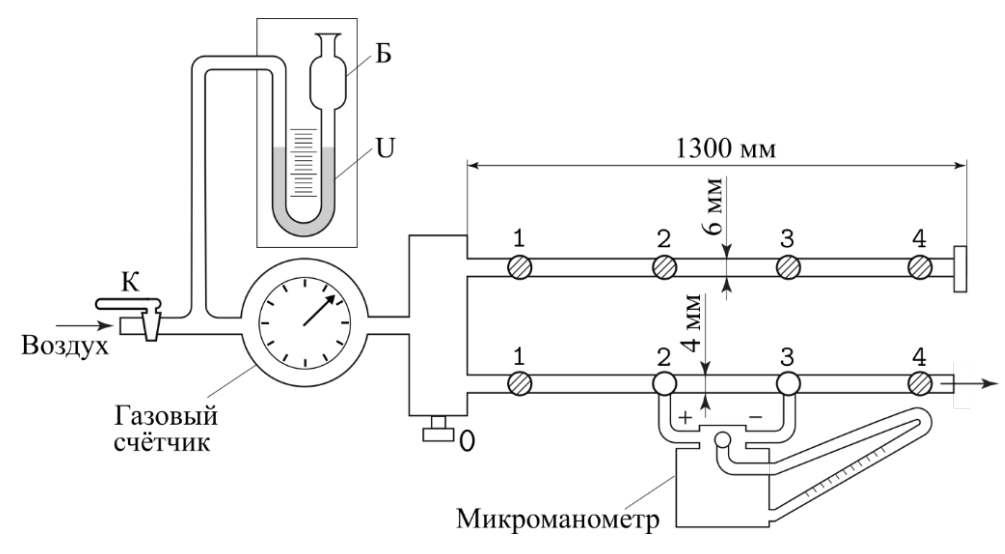
\includegraphics[scale=0.8]{рис 2.png}}
\caption{\textit{. Экспериментальная установка.}}
\end{figure}

\section*{3. Ход работы.}
\begin{itemize}
\item[\textbf{1. }] Подсоединим манометр к двум соседним выводам на трубке. Закроем все отверстия в этой и других трубках пробками, кроме выходного отверстия исследуемой трубки.

\noindent
Включаем компрессор. Переводим рычажок манометра в рабочее положение (+). Медленно приоткрывая кран K, создадим небольшой поток воздуха через трубу. Убеждаемся, что при неизменном положении крана K показания микроманометра стабильны, а стрелка расходомера вращается равномерно.

\item[\textbf{2. }] Измерим параметры окружающей среды: температуру, влажность воздуха и атмосферное давление. Запишем диаметры трубок. Результаты - в табл.1.

\begin{table}[h!]
\centering
\begin{tabular}{|c|c|c|c|c|c|}
\hline
$\varphi,   \%$ & $t, ^{\circ} \ C$ & $P_a, \text{ кПа}$ & $d_1$, см       & $d_2$, см       & $d_3$, см     \\ \hline
82              & 23.2              & 100               & 3.95 $\pm$ 0.05 & 5.05 $\pm$ 0.05 & 3.0 $\pm$ 0.1 \\ \hline
\end{tabular}
\caption{}
\end{table}
\item[\textbf{3. }] Проведём предварительные расчёты. Полагая критическое значение Re $\sim 10^{3}$, по формулам \eqref{eq4} определим критические значения расхода и разности давлений, при которых течение становится турбулентным:
\[Q_{cr} = \pi R^2 \frac{\eta Re}{\rho R} = \frac{\pi \eta Re R}{\rho}  \]
\[\Delta P_{cr} = \frac{8 \eta l}{R^2} \frac{\eta Re}{\rho R} = \frac{8 \eta^2 l Re}{\rho R^3} \]
Используя уравнение состояния идеального газа: $\rho = P \mu/(R_u T)$ (где $\mu = 0.029$ кг/моль - молярная масса воздуха), получим:
\begin{equation}\label{eq6}
Q_{cr} = \frac{\pi \eta Re R R_u T}{P \mu} 
\end{equation}
\begin{equation}\label{eq7}
\Delta P_{cr} = \frac{8 \eta^2 l Re}{R^3} \frac{R_u T}{P \mu}
\end{equation}

Значения $Q_{cr}$ и $\Delta P_{cr}$, а также $l_{est}$ (вычисляемое по формуле \eqref{eq5}) для всех трёх трубок - в табл. 2. При расчётах вязкость воздуха полагалась $\eta \sim 2 \cdot 10^{-5} \text{ Па} \cdot \text{с}$.

\noindent
Перевод давления из делений в Па осуществляется по формуле:
\[\Delta P = 0.2 \cdot g N \quad (N - \text{ число делений по шкале манометра})\]

\begin{table}[]
\centering
\begin{tabular}{|c|c|c|c|}
\hline
$d$, мм                   & 3.95  & 5.05  & 3.0   \\ \hline
$l$, см                   & 30    & 30    & 20    \\ \hline
$Q_{cr} \cdot 10^{3}$, л/c             & 105 & 135 & 80 \\ \hline
$\Delta P_{cr}$, Па       & 105.8 & 50.6  & 161.0 \\ \hline
$\Delta P_{cr}$, дел      & 54    & 26    & 82    \\ \hline
$\Delta P_{cr}^{exp}$, дел & 60    & 74    &       \\ \hline
$l_{est}$, см             & 39.5  & 50.5  & 30    \\ \hline
\end{tabular}
\caption{}
\end{table}

\item[\textbf{4. }] Меняя расход воздуха краном К и наблюдая за столбиком спирта в микроманометре, визуально определим границу перехода $\Delta P_{cr}$ от ламинарного течения к турбулентному.
Результаты - в табл. 2.
\item[\textbf{5. }] Так как относительная погрешность измерения расхода постоянна и равна $\varepsilon = 1\%$, то будем выбирать объём $V_{min}$ в зависимости от показаний секундомера. Выбор основан на том, что погрешность измерения времени (время реакции человека) $\sigma_t = 0.3$ с, поэтому чтобы погрешность измерения расхода $\Delta V/ \Delta t$, не превосходила $1 \%$, необходимо, чтобы $t \gtrsim 30$ с, что и будет достигаться выбором объёма.

\noindent
Погрешность измерения давления примем равной цене деления:
\[\sigma_{\Delta P} = 1 \text{ дел} = 2 \text{ Па} \]
\item[\textbf{6. }] Измерим зависимость $\Delta P (Q)$. Постепенно увеличивая расход, проведём измерения так, чтобы на ламинарный и турбулентный режимы приходилось по 7-9 точек. 

\noindent
Для измерения расхода будем измерять время $t$,  необходимое для прохождения объёма $V$ газа:
\[Q = \frac{V}{t} \quad ; \quad \sigma_Q = Q\sqrt{\varepsilon_V^2 + \left(\frac{\sigma_t}{t}\right)^2} \quad (\varepsilon_V = 1 \%) \]
Результаты - в табл. 3, 4, 5.
\begin{table}[]
\centering
\begin{tabular}{|c|c|c|c|c|c|c|}
\hline
V, л  & $\sigma_{V}$, л & $t$, с & $Q \cdot 10^{3}$, л/с & $\sigma_Q \cdot 10^{3}$, л/c & $\Delta P$, дел             & $\Delta P$, Па              \\ \hline
0.500 & 0.005           & 63.2   & 7.91                  & 0.09                         & \cellcolor[HTML]{00FF00}20  & \cellcolor[HTML]{00FF00}39  \\ \hline
1.000 & 0.010           & 55.7   & 17.9                  & 0.2                          & \cellcolor[HTML]{00FF00}25  & \cellcolor[HTML]{00FF00}49  \\ \hline
1.500 & 0.015           & 61.2   & 24.5                  & 0.3                          & \cellcolor[HTML]{00FF00}30  & \cellcolor[HTML]{00FF00}59  \\ \hline
1.500 & 0.015           & 50.2   & 29.9                  & 0.3                          & \cellcolor[HTML]{00FF00}35  & \cellcolor[HTML]{00FF00}69  \\ \hline
1.500 & 0.015           & 43.9   & 34.2                  & 0.4                          & \cellcolor[HTML]{00FF00}40  & \cellcolor[HTML]{00FF00}78  \\ \hline
2.00  & 0.02            & 46.3   & 43.2                  & 0.5                          & \cellcolor[HTML]{00FF00}45  & \cellcolor[HTML]{00FF00}88  \\ \hline
2.00  & 0.02            & 41.9   & 47.7                  & 0.6                          & \cellcolor[HTML]{00FF00}50  & \cellcolor[HTML]{00FF00}98  \\ \hline
2.50  & 0.03            & 48.4   & 51.7                  & 0.6                          & \cellcolor[HTML]{00FF00}55  & \cellcolor[HTML]{00FF00}108 \\ \hline
3.00  & 0.03            & 53.7   & 55.9                  & 0.6                          & \cellcolor[HTML]{00FF00}60  & \cellcolor[HTML]{00FF00}118 \\ \hline
3.00  & 0.03            & 50.2   & 59.8                  & 0.7                          & \cellcolor[HTML]{FF0000}65  & \cellcolor[HTML]{FF0000}128 \\ \hline
3.00  & 0.03            & 47.9   & 62.7                  & 0.7                          & \cellcolor[HTML]{FF0000}70  & \cellcolor[HTML]{FF0000}137 \\ \hline
3.00  & 0.03            & 45.4   & 66.0                  & 0.8                          & \cellcolor[HTML]{FF0000}75  & \cellcolor[HTML]{FF0000}147 \\ \hline
3.00  & 0.03            & 42.7   & 70.2                  & 0.9                          & \cellcolor[HTML]{FF0000}80  & \cellcolor[HTML]{FF0000}157 \\ \hline
3.50  & 0.04            & 46.9   & 74.7                  & 0.9                          & \cellcolor[HTML]{FF0000}85  & \cellcolor[HTML]{FF0000}167 \\ \hline
3.50  & 0.04            & 46.2   & 75.7                  & 0.9                          & \cellcolor[HTML]{FF0000}90  & \cellcolor[HTML]{FF0000}177 \\ \hline
3.50  & 0.04            & 43.7   & 80.1                  & 1.0                          & \cellcolor[HTML]{FF0000}95  & \cellcolor[HTML]{FF0000}186 \\ \hline
4.00  & 0.04            & 49.6   & 80.6                  & 0.9                          & \cellcolor[HTML]{FF0000}100 & \cellcolor[HTML]{FF0000}196 \\ \hline
\end{tabular}
\caption{. $d = 3.90$ мм}
\end{table}

\begin{table}[]
\centering
\begin{tabular}{|c|c|c|c|c|c|c|}
\hline
V, л & $\sigma_{V}$, л & $t$, с & $Q \cdot 10^{3}$, л/с & $\sigma_Q \cdot 10^{3}$, л/c & $\Delta P$, дел             & $\Delta P$, Па              \\ \hline
2.00 & 0.02            & 40.6   & 49.3                  & 0.6             & \cellcolor[HTML]{00FF00}35  & \cellcolor[HTML]{00FF00}69  \\ \hline
2.50 & 0.03            & 37.3   & 67.1                  & 0.9             & \cellcolor[HTML]{00FF00}40  & \cellcolor[HTML]{00FF00}78  \\ \hline
3.00 & 0.03            & 38.9   & 77.2                  & 1.0             & \cellcolor[HTML]{00FF00}45  & \cellcolor[HTML]{00FF00}88  \\ \hline
4.00 & 0.04            & 43.7   & 91.6                  & 1.1             & \cellcolor[HTML]{00FF00}50  & \cellcolor[HTML]{00FF00}98  \\ \hline
4.00 & 0.04            & 39.9   & 100.2                 & 1.3             & \cellcolor[HTML]{00FF00}55  & \cellcolor[HTML]{00FF00}108 \\ \hline
5.00 & 0.05            & 45.2   & 110.6                 & 1.3             & \cellcolor[HTML]{00FF00}60  & \cellcolor[HTML]{00FF00}118 \\ \hline
5.00 & 0.05            & 42.9   & 116.5                 & 1.4             & \cellcolor[HTML]{00FF00}65  & \cellcolor[HTML]{00FF00}128 \\ \hline
5.00 & 0.05            & 40.4   & 123.9                 & 1.5             & \cellcolor[HTML]{FF0000}70  & \cellcolor[HTML]{FF0000}137 \\ \hline
5.00 & 0.05            & 38.4   & 130.1                 & 1.7             & \cellcolor[HTML]{FF0000}75  & \cellcolor[HTML]{FF0000}147 \\ \hline
6.00 & 0.06            & 44.0   & 136.5                 & 1.7             & \cellcolor[HTML]{FF0000}80  & \cellcolor[HTML]{FF0000}157 \\ \hline
6.00 & 0.06            & 42.7   & 140.5                 & 1.7             & \cellcolor[HTML]{FF0000}85  & \cellcolor[HTML]{FF0000}167 \\ \hline
6.00 & 0.06            & 40.6   & 147.9                 & 1.8             & \cellcolor[HTML]{FF0000}90  & \cellcolor[HTML]{FF0000}177 \\ \hline
6.00 & 0.06            & 39.6   & 151.4                 & 1.9             & \cellcolor[HTML]{FF0000}95  & \cellcolor[HTML]{FF0000}186 \\ \hline
6.00 & 0.06            & 38.5   & 155.9                 & 2.0             & \cellcolor[HTML]{FF0000}100 & \cellcolor[HTML]{FF0000}196 \\ \hline
\end{tabular}
\caption{. $d = 5.05$ мм}
\end{table}

\begin{table}[]
\centering
\begin{tabular}{|c|c|c|c|c|c|c|}
\hline
V, л  & $\sigma_{V}$, л & $t$, с & $Q \cdot 10^{3}$, л/с & $\sigma_Q$, л/c & $\Delta P$, дел             & $\Delta P$, Па              \\ \hline
6.00  & 0.06            & 33.1   & 181                   & 2               & \cellcolor[HTML]{00FF00}70  & \cellcolor[HTML]{00FF00}137 \\ \hline
7.00  & 0.07            & 34.9   & 200                   & 3               & \cellcolor[HTML]{00FF00}80  & \cellcolor[HTML]{00FF00}157 \\ \hline
10.00 & 0.10            & 37.5   & 267                   & 3               & \cellcolor[HTML]{00FF00}130 & \cellcolor[HTML]{00FF00}255 \\ \hline
\end{tabular}
\caption{. $d = 3.0$ мм}
\end{table}

\item[\textbf{7. }] Измерим распределение давления газа вдоль трубки $P(x)$. Установим поток воздуха через трубку, близкий к критическому, но всё ещё сохраняющий ламинарность. Не меняя расхода, последовательно подсоединим микроманометр ко всем парам выводов исследуемой трубки. Вывод "0"\ примем за начало отсчёта. Значения давления на одинаковых расстояниях $x$ будем усреднять. Результаты - в табл. 6, 7, 8, 9.

\begin{table}[]
\begin{minipage}{0.49\linewidth}
\centering
\begin{tabular}{|c|c|c|c|}
\hline
$L$, см & $\Delta P$, дел & $i$ & $j$ \\ \hline
11.5    & 20              & 0   & 1   \\ \hline
41.5    & 70              & 0   & 2   \\ \hline
81.5    & 98              & 0   & 3   \\ \hline
131.5   & 132             & 0   & 4   \\ \hline
30.0    & 50              & 1   & 2   \\ \hline
70.0    & 77              & 1   & 3   \\ \hline
120.0   & 112             & 1   & 4   \\ \hline
40.0    & 45              & 2   & 3   \\ \hline
90.0    & 99              & 2   & 4   \\ \hline
50.0    & 54              & 3   & 4   \\ \hline
\end{tabular}
\caption{. \newline $d = 3.95$ мм \newline $Q = 47.7 \cdot 10^{-3}$ л/c}
\end{minipage}
\begin{minipage}{0.49\linewidth}
\centering
\begin{tabular}{|c|c|}
\hline
$x$, см & $\Delta P(x)$, Па \\ \hline
11.5    & 39                \\ \hline
41.5    & 137               \\ \hline
81.5    & 192               \\ \hline
131.5   & 259               \\ \hline
\end{tabular}
\caption{. \newline $d = 3.95$ мм \newline $Q = 47.7 \cdot 10^{-3}$ л/c}
\end{minipage}
\end{table}

\begin{table}[]
\begin{minipage}{0.49\linewidth}
\centering
\begin{tabular}{|c|c|c|c|}
\hline
$L$, см & $\Delta P$, дел & $i$ & $j$ \\ \hline
11.5    & 46              & 0   & 1   \\ \hline
41.5    & 64              & 0   & 2   \\ \hline
81.5    & 97              & 0   & 3   \\ \hline
131.5   & 126             & 0   & 4   \\ \hline
30.0    & 37              & 1   & 2   \\ \hline
70.0    & 70              & 1   & 3   \\ \hline
120.0   & 97              & 1   & 4   \\ \hline
40.0    & 49              & 2   & 3   \\ \hline
90.0    & 79              & 2   & 4   \\ \hline
50.0    & 54              & 3   & 4   \\ \hline
\end{tabular}
\caption{. \newline $d = 5.05$ мм \newline $Q = 124 \cdot 10^{-3} $ л/c}
\end{minipage}
\begin{minipage}{0.49\linewidth}
\centering
\begin{tabular}{|c|c|}
\hline
$x$, см & $\Delta P$, Па \\ \hline
11.5    & 90            \\ \hline
41.5    & 144           \\ \hline
81.5    & 190           \\ \hline
131.5   & 247           \\ \hline
\end{tabular}
\caption{. \newline $d = 5.05$ мм \newline $Q = 124 \cdot 10^{-3} $ л/c}
\end{minipage}
\end{table}
\item[\textbf{8. }] По данным табл. 3-5 построим графики зависимости $Q(\Delta P)$ для трёх трубок. Результаты - на рис. 3, 4, 5. Аппроксимируем результаты по МНК. Для коэффициента пропорциональности $Q(\Delta P)$ получим ($d = 3.95$ мм):
\[\alpha \equiv \frac{\pi R^4}{8 \eta l} = (0.67 \pm 0.03) \cdot 10^{-6} \frac{\text{м}^3}{\text{Па} \cdot \text{с}} \Rightarrow \eta = \frac{\pi R^4}{8 \alpha l} = (3.1 \pm 0.2) \cdot 10^{-5} \text{ Па} \cdot \text{с} \]

\noindent
Для $d = 5.05$ мм:
\[\alpha =  (1.10 \pm 0.07) \cdot 10^{-6} \frac{\text{м}^3}{\text{Па} \cdot \text{с}} \Rightarrow \eta = (4.7 \pm 0.2) \cdot 10^{-5} \text{ Па} \cdot \text{с}\]

\noindent
Для $d = 3.0$ мм:
\[\alpha =  (0.72 \pm 0.05) \cdot 10^{-6} \frac{\text{м}^3}{\text{Па} \cdot \text{с}} \Rightarrow \eta = (1.4 \pm 0.9) \cdot 10^{-5} \text{ Па} \cdot \text{с}\]


\begin{figure}
\center{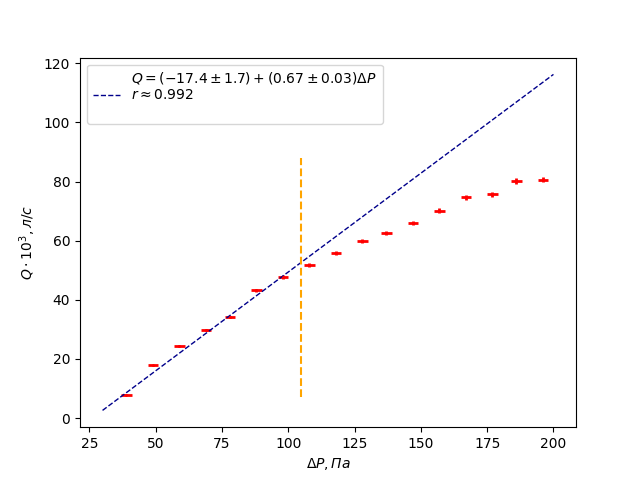
\includegraphics[scale=1]{рис 3.png}}
\caption{. $d = 3.95$ мм}
\end{figure}

\begin{figure}
\center{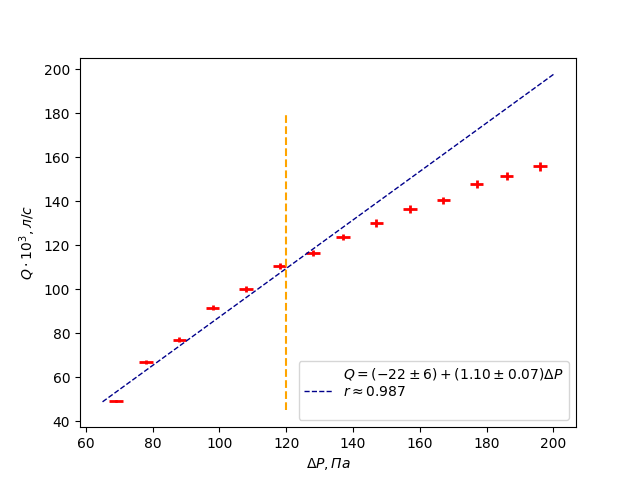
\includegraphics[scale=1]{рис 4.png}}
\caption{. $d = 5.05$ мм}
\end{figure}

\begin{figure}
\center{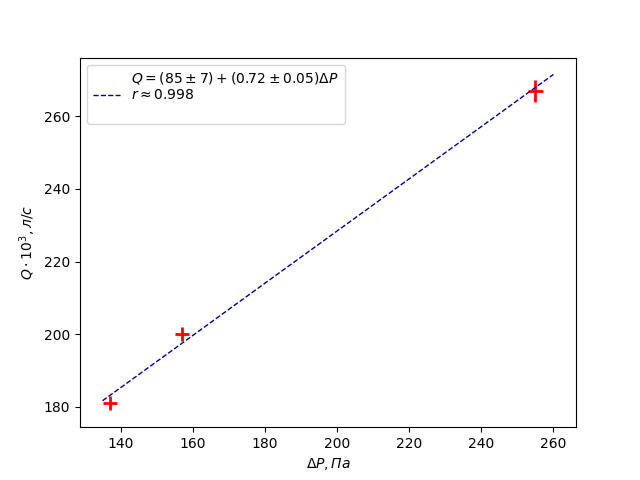
\includegraphics[scale=1]{рис 5.png}}
\caption{. $d = 3.0$ мм}
\end{figure}

\noindent
По графикам определяем, что для трубки диаметром $d = 3.95$ мм переход от ламинарного к турбулентному участку происходит при:
\[\Delta P_{cr} \approx 105 \text{ Па} \quad ; \quad Q_{cr} \approx 50 \cdot 10^{-3} \text{ л/c} \]
Для трубки с $d = 5.05$ мм:
\[\Delta P_{cr} \approx 120 \text{ Па} \quad ; \quad Q_{cr} \approx 110 \cdot 10^{-3} \text{ л/с} \]
Из формул \eqref{eq6}, \eqref{eq7} можно определить критическое число Рейнольдса по критическим значениям $\Delta P_{cr}$ и $Q_{cr}$. Для трубки $d = 3.95$ мм:
\[Re_{Q} = \frac{P \mu Q_{cr}}{\pi \eta R R_u T} \approx 312 \ ; \ Re_{\Delta P} = \frac{P \mu R^3 \Delta P_{cr}}{8\eta^2 l R_u T} \approx 396 \ ; \ Re_{\Delta P^{exp}} \approx 410\] 

\noindent
Для трубки с $d = 5.05$ мм:
\[Re_{Q} \approx 350 \ ; \  Re_{\Delta P} \approx 415 \ ; Re_{\Delta P^{exp}} \approx 505 \]
Полученные значения $Re$ близки между собой, однако в 2 раза отличаются от предполагаемого изначально значения.
\item[\textbf{9.}] По данным табл. 7, 9 построим график зависимости падения давления $\Delta P(x)$ для трубок с $d = 3.95$ мм и $d = 5.05$ мм. Результаты - на рис. 6, 7.

\noindent
Как видно, зависимости являются линейными, а градиенты давления в пределах погрешностей совпадают. Определить длину установления ламинарного течения по этим зависимостям невозможно, т.к. мало экспериментальных точек.
\end{itemize}
\begin{figure}
\center{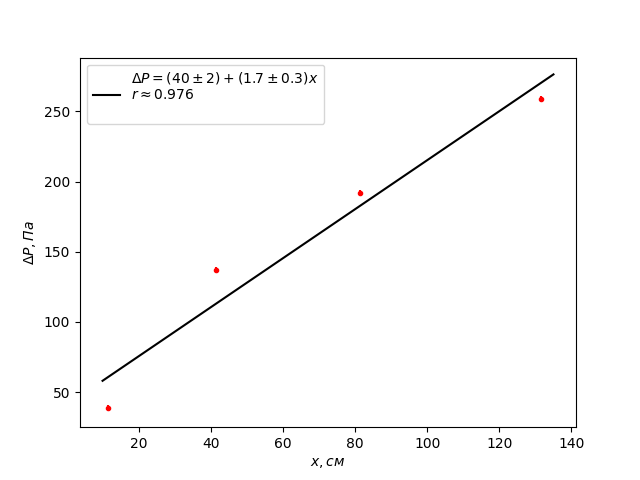
\includegraphics[scale=1]{рис 6.png}}
\caption{. $d = 3.95$ мм}
\end{figure}
\begin{figure}
\center{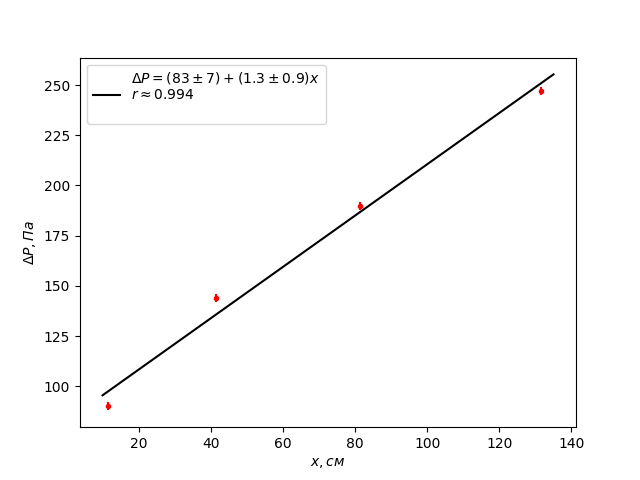
\includegraphics[scale=1]{рис 7.png}}
\caption{. $d = 5.05$ мм}
\end{figure}
\section*{4. Вывод.}
В работе были исследованы свойства течения воздуха по трубкам различного диаметра при различных числах рейнольдса. Было выяснено, что закон Пуазейля применим при числах Рейнольдса $Re \lesssim 400$. Это значение подтверждается анализом зависимости расхода от разности давлений для разных трубок, а также прямыми измерениями по наблюдению за колебаниями столбика микроманометра.

\noindent
В работе был проверен закон Пуазейля для ламинарного течения путём анализа зависимости $Q(\Delta P)$. Из той же зависимости были определены значения вязкости воздуха:
\[\eta_1 =  (3.1 \pm 0.2) \cdot 10^{-5} \text{ Па} \cdot \text{с} \ ; \ \eta_2 = (4.7 \pm 0.2) \cdot 10^{-5} \text{ Па} \cdot \text{с}\]
Полученные значения выше табличного для $t = 21.3 \ ^{\circ}C$, $P = 10^{5}$ Па:
\[\eta_0 = 2.06 \cdot 10^{-5} \text{ Па} \cdot \text{с} \]
\end{document}
